\documentclass[fem.tex]{subfiles}

\begin{document}
\section{Generation of Finite Mesh}%
\label{sec:generation_of_finite_mesh}

The first stage in the computational process of FEM, is to generate the finite
mesh over the domain of the problem. There are several different methods that
can be used to generate the mesh, the method that this paper utilizes is
Delaunay triangulation. An alternative that is less utilized is the method of
polygon clipping. The scope of this paper is restricted to two
dimensional domains. However, the method for mesh generation is easily
generalizable to higher dimensions.

The generation of a mesh using Delaunay triangulation has several stages.

\begin{enumerate}
  \item Delaunay triangulation
  \item Applying boundaries
  \item Mesh refinement
\end{enumerate}

\subsection{Delaunay Triangulation}%
\label{sub:delaunay_triangulation}

A Delaunay triangulation for a set of points $P$ is a triangulation $DP(P)$
such that no point in $P$ is in the circumcircle of any triangle in the
triangulation $DP(P)$. This form of triangulation maximizes the minimum angle
of all triangles in the triangulation, thus avoiding sliver triangles. See
Fig ~\ref{fig:delaunay_triangulation} for an example of Delaunay Triangulation.

\begin{Figure}
\begin{center}
  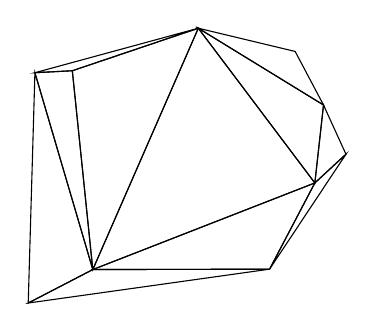
\begin{tikzpicture}[scale=0.5]
    
\draw[black] (2.17,6.47)--(2.69,1.42)--(5.37,7.55)--cycle;
\draw[black] (7.83,6.96)--(5.37,7.55)--(8.55,5.6)--cycle;
\draw[black] (8.33,3.62)--(5.37,7.55)--(2.69,1.42)--cycle;
\draw[black] (8.33,3.62)--(2.69,1.42)--(7.18,1.43)--cycle;
\draw[black] (8.33,3.62)--(8.55,5.6)--(5.37,7.55)--cycle;
\draw[black] (1.05,0.57)--(7.18,1.43)--(2.69,1.42)--cycle;
\draw[black] (1.22,6.42)--(2.17,6.47)--(5.37,7.55)--cycle;
\draw[black] (1.22,6.42)--(1.05,0.57)--(2.69,1.42)--cycle;
\draw[black] (1.22,6.42)--(2.69,1.42)--(2.17,6.47)--cycle;
\draw[black] (9.12,4.35)--(8.33,3.62)--(7.18,1.43)--cycle;
\draw[black] (9.12,4.35)--(8.55,5.6)--(8.33,3.62)--cycle;
\end{tikzpicture}
\end{center}
\captionof{figure}{Example of Delaunay Triangulation}
\label{fig:delaunay_triangulation}
\end{Figure}

The generation of the Delaunay triangulation has several different algorithms,
and is constantly advancing in efficiency. There are three main algorithms that
are documented for the generation of the triangulation.

\begin{enumerate}
  \item Edge flipping
  \item Incremental
  \item Divide and conquer
\end{enumerate}

It is important to note that each algorithm will produce the same resulting
triangulation. This is due to the fact that the Delaunay triangulation
associated with a set of points is unique, with one exceptions of the points on
a square.

\subsubsection{Edge Flipping}%
\label{ssub:edge_flipping}

This method for generating the Delaunay triangulation, is a very simple
algorithm, and not very efficient.

\subsubsection{Incremental}%
\label{ssub:incremental}

This method for generating the Delaunay triangulation is better than the
\ref{ssub:edge_flipping} algorithms, but can still be improved upon.

The basis of this method, is to incrementaly add the points from $P$ to the
triangulation, and regenerate the triangles that that point is within the
circumcircle of.

The steps of the algorithm are detailed below. which is then followed by
psudocode.

\begin{enumerate}
  \item Generate a bounding triangle, such that all points in $P$ are within
    the triangle. Append the points of this bounding triangle to the end of
    $P$.
  \item For every point in $P$ do 3-6
  \item Select $p$ from $P$
  \item For every triangle in $DT(P)$ if $p$ is within the circumcircle of that
    triangle add that triangle to a list of bad triangles $BT$ and remove that
    triangle from $DT(P)$.
  \item For every triangle in $BT$, add every edge of the triangle to a polygon
    $Poly$, only if that edge is not shared by any other triangles in $BT$.
  \item For every edge in $Poly$ create a new triangle by connecting that edge
    to $p$.
  \item Remove all triangles from $DT(P)$ if one of the verticies is one of the
    three generated in step 1.
\end{enumerate}

\subsubsection{Divide and Conquer}%
\label{ssub:divide_and_conquer}

This algorithm for constructing the Delaunay triangulation is currently shown
to be the fastest, and allows for optimization in computational execution
that the previous algorithms lacked.

This algorithm allows for easy parallelism in the computation of the
triangulation, thus allowing computers to calculate the triangulation much more
efficiently than the other algorithms permit.

\subsection{Applying Boundaries}%
\label{sub:applying_boundaries}

Now that the Delaunay triangulation has been generated, the next stage is to
apply the constraints of the boundary conditions to the triangulation.

\subsection{Mesh Refinement}%
\label{sub:mesh_refinement}

The final stage is to refine the mesh, because the restriction of the boundary
conditions are able to cause non-delaunay triangles. This stage also applies
larger restrictions to the triangles, resulting is ``nicer'' triangles with
restricted minimum angles.

\end{document}
